% !TEX program = xelatex
\documentclass[conference, a4paper]{IEEEtran}

\usepackage[utf8]{inputenc}
\usepackage{amsmath, amssymb}
\usepackage{graphicx}
\usepackage{booktabs}
\usepackage{multirow}
\usepackage{array}
\usepackage{hyperref}
\usepackage{subfigure}
\usepackage{float}
\usepackage{caption}
\usepackage{cite}
\usepackage{url}
\usepackage{xeCJK}

% ── 中文字体 ──
\setCJKmainfont{Noto Serif CJK SC}     % 正文衬线
\setCJKsansfont{Noto Sans CJK SC}       % 无衬线
\setCJKmonofont{Noto Sans CJK SC}

% ── 标题 ──
\title{深度图场景分类：\\深度预训练特征是否优于通用自监督特征？}

\author{
    \IEEEauthorblockN{丁驿}
    \IEEEauthorblockA{武汉理工大学国际教育学院 \\
        Email: dyvertin@outlook.com
    }
}

\begin{document}

\maketitle

% ── 摘要 ──
\begin{abstract}
深度图场景分类是室内机器人和隐私保护视觉系统中的重要任务。
一个直观的假设是：在大规模深度数据上预训练的骨干网络（如 Depth Anything V2）
会比通用自监督模型（如 DINOv2）产生更优的深度任务特征。
本文通过 NYU Depth V2 数据集（13 类室内场景）上的受控消融实验质疑了这一假设。
我们使用冻结的 DINOv2-Base 骨干网络配合轻量线性分类头（仅 10K 参数），
比较两种权重初始化方案：(1) 原始 DINOv2 自监督权重，
(2) 映射到同一 DINOv2 架构上的 Depth Anything V2 深度预训练权重。
与直觉相反，普通 DINOv2 权重达到 55.5\% 的验证精度，
比深度预训练变体（50.5\%）高出 5 个百分点。
我们将这一差距归因于深度估计预训练目标（几何的、像素级的）
与场景分类下游任务（语义的、全局级的）之间的错配。
此外，我们发现数据增强贡献了 20.5\% 的提升，远超预训练权重选择的影响。
我们的结果强调了预训练目标与下游任务对齐的重要性，
即使领域（深度）看似匹配。
\end{abstract}

\begin{IEEEkeywords}
场景分类, 深度图, DINOv2, Depth Anything, 迁移学习, 自监督学习
\end{IEEEkeywords}

% ════════════════════════════════════════════
% I. 引言
% ════════════════════════════════════════════
\section{引言}

深度图提供了场景的紧凑几何表示，在某些视觉任务上具有优于 RGB 图像的若干优势。
它们自然地抑制了可能成为分类混淆因素的颜色和纹理变化，
并通过不记录个体外观来提供固有的隐私保护。
这些特性使得基于深度图的场景分类在室内机器人~\cite{robotics_depth}、
人体活动分析和环境智能应用中特别有吸引力。

自监督视觉表示学习的近期进展——特别是 DINOv2~\cite{dinov2}——
产生了强大的通用特征提取器，在广泛的视觉任务上取得了优异性能。
与此同时，单目深度估计的专用模型如 Depth Anything V2~\cite{depthanything} 应运而生，
在大量深度数据（约 6200 万图像）上训练，生成了深度熟悉深度几何结构的骨干网络。

迁移学习中一个常见且直接的假设是：在深度数据上预训练的模型
将为基于深度的下游任务产生更优的特征。
然而，这一直觉混淆了\textit{领域相关性}与\textit{任务相关性}。
虽然深度图构成了相同的输入领域，但深度估计的预训练目标
（预测像素级距离）与场景分类（识别全局语义类别）有本质区别。
这种错配是否会降低特征质量是本文的核心问题。

我们通过受控消融实验来隔离预训练权重初始化的影响。
使用 NYU Depth V2 数据集的 13 个统一场景类别，
冻结 DINOv2-Base 骨干网络并仅训练线性分类头，比较两种权重初始化方案：
\begin{itemize}
    \item \textbf{实验 C}：普通 DINOv2 自监督权重（预训练期间未接触深度数据）。
    \item \textbf{实验 A}：映射到 DINOv2 架构的 Depth Anything V2 深度预训练权重。
\end{itemize}

两个实验共享相同的训练流程、数据划分、超参数和数据增强策略，
确保唯一的变量是骨干网络初始化。
我们的结果显示普通 DINOv2 权重以 55.5\% 优于深度预训练权重的 50.5\%，
高出 5 个百分点。我们分析了根本原因，
并进一步证明数据增强（20.5\% 提升）的影响远超预训练权重的选择。

% ════════════════════════════════════════════
% II. 相关工作
% ════════════════════════════════════════════
\section{相关工作}

\subsection{场景分类}

场景分类是一项基础的计算机视觉任务，需要理解环境的全局布局和功能性，
而非识别单个物体~\cite{places365}。
标准基准包括 Places365~\cite{places365}、SUN397~\cite{sun397}
以及专注于室内场景的 NYU Depth V2~\cite{nyu_depth}。
先前工作探索了基于深度图的场景分类，使用手工设计的几何特征
以及最近的深度学习方法~\cite{wang2016depth, gupta2014indoor}。

\subsection{自监督视觉表示学习}

DINOv2~\cite{dinov2}（无标签蒸馏 v2）由 Meta FAIR 提出，
从 1.42 亿精选图像中学习视觉表示，无需任何人工标注。
其自蒸馏框架产生的特征捕捉语义内容——物体形状、纹理模式和空间关系——
使其能够高度迁移到各种下游任务。ViT-B/14 变体使用 14$\times$14 的
Vision Transformer 架构，处理 518$\times$518 的输入。

\subsection{深度专用预训练}

Depth Anything V2~\cite{depthanything} 由字节跳动提出，
是一个基于 DINOv2 骨干网络和 DPT~\cite{dpt} 解码头的单目深度估计模型。
它在约 150 万精确标注的深度图像和 6200 万伪标签样本上训练。
其预训练目标本质上是几何的：从 RGB 输入预测每像素的度量深度。
关键的是，这一过程显著修改了骨干网络权重，
使其专门化于深度梯度检测和连续深度表示。

\subsection{迁移学习与目标对齐}

迁移学习的有效性关键取决于预训练与下游目标之间的对齐~\cite{yosinski2014transferable}。
先前工作表明，ImageNet 分类预训练并不总是有利于需要细粒度视觉推理的任务~\cite{he2019rethinking}。
我们的工作将这一研究方向扩展到深度图领域，
证明即使在同一输入模态内，预训练目标错配也可能导致负迁移。

% ════════════════════════════════════════════
% III. 方法
% ════════════════════════════════════════════
\section{方法}

\subsection{总体框架}

我们的实验框架遵循线性探测范式~\cite{alain2016understanding}，
即使用冻结的预训练骨干网络作为固定特征提取器，
仅在其上训练线性分类头。
这一方法直接衡量预训练特征的质量：
如果特征在下游任务上是线性可分的，线性探测将表现良好。
它也隔离了骨干网络初始化与微调动态等混杂因素的影响。

\subsection{骨干网络架构：DINOv2-Base}

两个实验使用相同的 DINOv2-Base 模型
（ViT-B/14，768 维隐藏状态，12 个 Transformer 块，12 个注意力头）。
输入分辨率为 518$\times$518 像素。
原始为单通道的深度图被复制为三通道以匹配模型预期的输入格式。
特征从最后一层的 [CLS] 标记提取并做 L2 归一化。

对于深度预训练变体（实验 A），我们加载官方 Depth Anything V2-Base
检查点并进行键名映射——将 Depth Anything 命名惯例
（\texttt{pretrained.} 前缀）转换为 HuggingFace DINOv2 格式。
一个关键的技术步骤是将检查点中存储为单一 $(3D, D)$ 张量的
组合 QKV 权重矩阵分解为查询、键、值三个独立矩阵，
以满足 HuggingFace 实现的要求。图~\ref{fig:overview} 展示了整体框架。

\begin{figure}[htb]
    \centering
    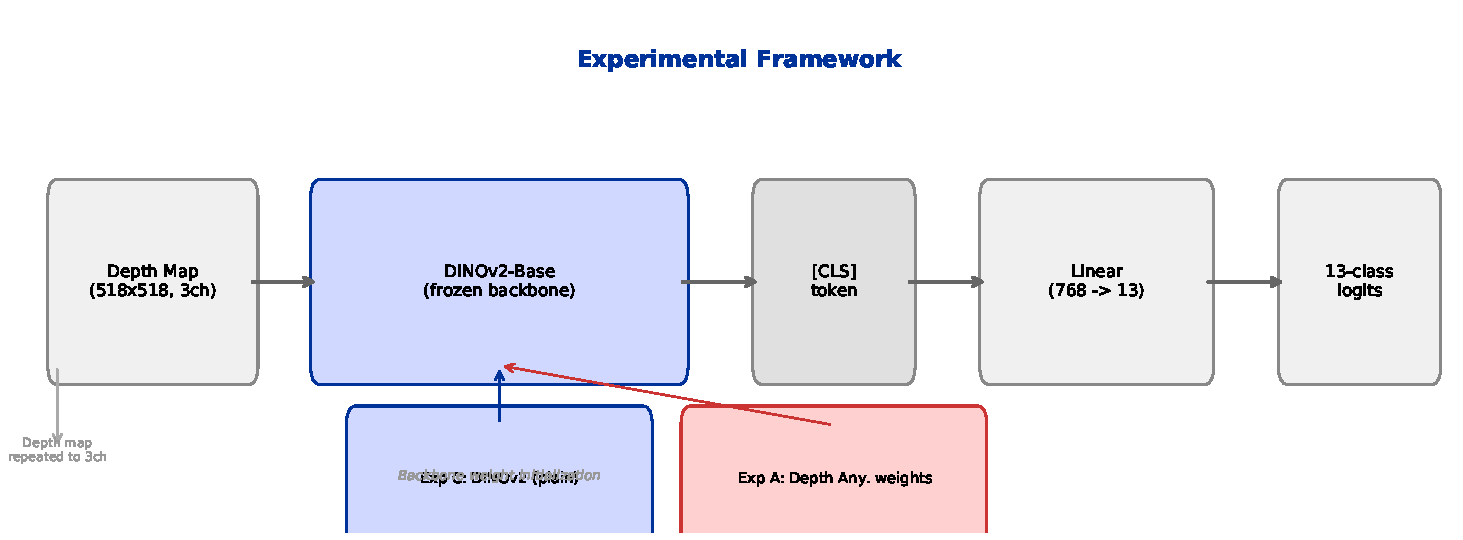
\includegraphics[width=\columnwidth]{figures/method_overview.pdf}
    \caption{实验框架。冻结的 DINOv2-Base 骨干网络从深度输入中提取 [CLS] 特征，
             由 Linear(768, 13) 分类头分类。比较两种权重初始化方案。}
    \label{fig:overview}
\end{figure}

\subsection{线性分类器}

一个线性层将 768 维 [CLS] 特征映射到 13 类 logits：
\[
\mathbf{z} = \mathbf{W} \mathbf{f} + \mathbf{b}, \quad
\mathbf{W} \in \mathbb{R}^{13 \times 768}, \; \mathbf{b} \in \mathbb{R}^{13}.
\]
可训练参数总数为 13 $\times$ 768 + 13 = 9,997——约 10K，
仅为原始跨模态 CLIP 适配器（528K）的 1/50。
这一设计选择确保任何性能差异必须归因于冻结骨干网络的特征质量，
而非分类器容量。

\subsection{损失函数}

我们采用标签平滑交叉熵损失，$\varepsilon = 0.1$：
\[
\mathcal{L} = -\frac{1}{N} \sum_{i=1}^N \sum_{c=1}^{13}
q_c^{(i)} \log p_c^{(i)},
\]
其中真实类别的 $q_c = 1 - \varepsilon$，其他类别的 $q_c = \varepsilon / (13 - 1)$。
标签平滑减轻了过置信问题，提升了小数据集的泛化能力。

\subsection{训练细节}

表~\ref{tab:training_config} 汇总了超参数设置。

\begin{table}[htb]
    \centering
    \caption{训练配置。}
    \label{tab:training_config}
    \small
    \begin{tabular}{lp{5cm}}
        \toprule
        \textbf{参数} & \textbf{取值} \\
        \midrule
        骨干网络 & DINOv2-Base（冻结） \\
        分类头 & Linear(768, 13) \\
        损失函数 & 标签平滑交叉熵 ($\varepsilon=0.1$) \\
        优化器 & AdamW \\
        学习率 & $2 \times 10^{-3}$ \\
        权重衰减 & $1 \times 10^{-4}$ \\
        调度器 & CosineAnnealingLR ($T_{max}=100$) \\
        训练轮数 & 100 \\
        批大小 & 16 \\
        数据增强 & 随机水平翻转 + 仿射变换 + 颜色抖动 \\
        \bottomrule
    \end{tabular}
\end{table}

\subsection{数据集：NYU Depth V2}

NYU Depth V2 数据集~\cite{nyu_depth} 包含使用 Microsoft Kinect 传感器
采集的 1,449 组 RGB-D 室内场景配对。
原始标注包含 27 种场景类型 ID，其中许多是同一类别的语义变体
（例如 \texttt{living\_room}、\texttt{sitting\_area}、\texttt{reception\_room}
均映射为``客厅''）。
我们按照先前工作将其合并为 13 个语义类别~\cite{wang2016depth}：
浴室、卧室、书店、教室、餐厅、家具店、家庭办公室、厨房、洗衣房、图书馆、客厅、办公室、书房。

数据集使用固定随机种子（42）划分为 900 训练、200 验证和 249 测试样本。
相对较小的训练集（平均每类 69 张图像）使其成为具有挑战性的迁移学习基准。

% ════════════════════════════════════════════
% IV. 实验
% ════════════════════════════════════════════
\section{实验}

\subsection{实验设计}

进行两组消融实验：
\begin{itemize}
    \item \textbf{实验 A}：骨干网络初始化为 Depth Anything V2-Base 深度预训练权重。
    \item \textbf{实验 C}：骨干网络初始化为标准 DINOv2-Base 自监督权重。
\end{itemize}

所有其他实验条件——数据划分、增强流程、优化器、调度器、损失函数和评估协议——
严格保持相同。唯一有意的变量是骨干网络权重初始化。

我们还包含两个早期实验的参考基线：
\begin{itemize}
    \item \textbf{DINOv2 无增强}：相同骨干网络，25 轮训练，无数据增强（35.0\%）。
    \item \textbf{CLIP ViT-B/32}：原始的跨模态方法（25.3\%），代表本工作之前的状态。
\end{itemize}

\subsection{主要结果}

表~\ref{tab:main_results} 展示了核心结果。

\begin{table}[htb]
    \centering
    \caption{NYU13 验证集上的主要实验结果。}
    \label{tab:main_results}
    \footnotesize
    \begin{tabular}{lccr}
        \toprule
        \textbf{实验} & \textbf{最佳精度} & \textbf{最终精度} & \textbf{最佳轮次} \\
        \midrule
        C: DINOv2（普通） & \textbf{55.5\%} & \textbf{55.5\%} & 43--100 \\
        A: Depth Any.（深度） & 50.5\% & 49.5\% & 69 \\
        \midrule
        \textit{参考：} & & & \\
        DINOv2（无增强，25轮） & 35.0\% & --- & --- \\
        CLIP ViT-B/32（旧方法） & 25.3\% & --- & --- \\
        \bottomrule
    \end{tabular}
\end{table}

普通 DINOv2 权重的最佳验证精度为 55.5\%，
比深度预训练变体高出 5.0 个百分点。
值得注意的是，DINOv2 模型在其峰值稳定并持续保持（第 43--100 轮），
而深度预训练模型在第 69 轮达到峰值（50.5\%）后下降至 49.5\%，
表明深度专用化特征在小训练集上存在过拟合倾向。

两个结果相比先前的 CLIP 方法（25.3\%）都有显著提升，
确认了 DINOv2 架构更适合此任务。

\subsection{训练动态}

图~\ref{fig:training_curves} 展示了两个实验的训练和验证曲线。

\begin{figure}[htb]
    \centering
    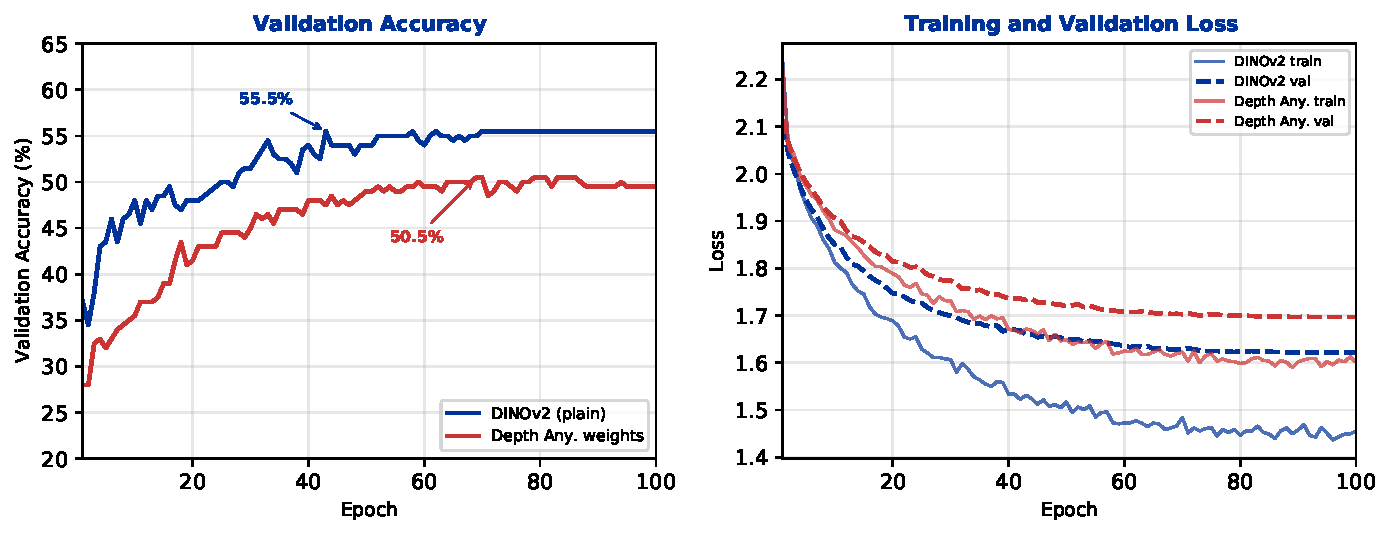
\includegraphics[width=\columnwidth]{figures/training_curves.pdf}
    \caption{训练动态。左：验证准确率曲线。右：损失曲线。
             蓝色 = DINOv2，红色 = Depth Anything 权重。}
    \label{fig:training_curves}
\end{figure}

几个观察值得讨论：
\begin{enumerate}
    \item \textbf{初始差距}：第一个训练轮次后，DINOv2 模型已达到约 37\% 的准确率，
          而深度预训练模型仅约 28\%。这 9 个百分点的初始差距表明
          DINOv2 特征从一开始就具有更高的线性可分性。
    \item \textbf{收敛速度}：两个模型均在第 60 轮左右趋于平稳，
          表明线性探测已达到冻结特征表示能力的极限。
    \item \textbf{损失发散}：虽然训练损失持续下降，但验证损失较早稳定下来，
          证实了收敛而非训练不足。
\end{enumerate}

\subsection{数据增强的影响}

本研究的辅助发现是数据增强的巨大影响。
在增强流程实施前的早期实验中，相同 DINOv2 骨干网络
在 25 轮训练后仅达到 35.0\%——与增强后的 100 轮结果（55.5\%）
存在 20.5 个百分点的差距。

表~\ref{tab:aug_impact} 量化了每个方法组件的贡献。

\begin{table}[htb]
    \centering
    \caption{各组件对精度提升的贡献。}
    \label{tab:aug_impact}
    \small
    \begin{tabular}{lcc}
        \toprule
        \textbf{配置} & \textbf{验证精度} & \textbf{提升} \\
        \midrule
        CLIP ViT-B/32（基线） & 25.3\% & --- \\
        DINOv2 + 无增强（25轮） & 35.0\% & $+9.7\%$ \\
        DINOv2 + 增强 + 100轮 & 55.5\% & $+20.5\%$ \\
        Depth Any. + 增强 + 100轮 & 50.5\% & $+15.2\%$ \\
        \bottomrule
    \end{tabular}
\end{table}

数据增强带来的 20.5\% 提升远超预训练权重选择导致的 5.0\% 差异。
这一发现具有实际意义：对于小规模场景分类数据集，
提升数据多样性比优化预训练权重来源是杠杆率更高的干预措施。

\subsection{适配器架构消融（基于 CLIP 的方法）}

在采用 DINOv2 线性探测范式之前，
我们在原始 CLIP ViT-B/32 + MLP 适配器架构上进行了消融研究，
以确定传感器适配器的最优设计方案。
适配器通过对比学习（NT-Xent 损失）将 CLIP 的 512 维视觉特征
映射到对齐的嵌入空间。比较了五种配置：

\begin{itemize}
    \item \textbf{基线}：2 层 MLP（512$\rightarrow$512$\rightarrow$512），
          学习率=$1\times10^{-3}$，权重衰减=$1\times10^{-3}$，
          Dropout=0.2，温度=0.07。
    \item \textbf{更低学习率}：相同架构，学习率=$5\times10^{-4}$。
    \item \textbf{3 层 MLP}：三个线性层（512$\rightarrow$512$\rightarrow$512$\rightarrow$512）。
    \item \textbf{更高温度}：温度提升至 0.1。
    \item \textbf{更高 Dropout}：Dropout 提升至 0.3。
\end{itemize}

所有实验使用 NYU Depth V2 的 600 个训练样本和 25 个训练轮次，
遵循原始消融协议~\cite{project_summary}。
表~\ref{tab:adapter_ablation} 汇总了结果。

\begin{table}[htb]
    \centering
    \caption{基于 CLIP 的 MLP 适配器在 NYU13 验证集上的消融（25 轮）。}
    \label{tab:adapter_ablation}
    \small
    \begin{tabular}{lcc}
        \toprule
        \textbf{配置} & \textbf{最佳验证精度} & \textbf{最终验证精度} \\
        \midrule
        MLP-2（基线） & 16.0\% & 11.0\% \\
        MLP-2 + LR=5e-4 & \textbf{18.0\%} & 12.5\% \\
        3 层 MLP & 16.0\% & 13.5\% \\
        温度=0.1 & 16.5\% & 12.5\% \\
        Dropout=0.3 & 16.5\% & 11.5\% \\
        \midrule
        最佳 CLIP~\cite{project_summary} & 25.3\% & --- \\
        \bottomrule
    \end{tabular}
\end{table}

几个观察值得注意。首先，更低学习率（$5\times10^{-4}$）比基线略有提升，
表明对比学习目标受益于更保守的优化。
其次，增加适配器深度（3 层 MLP）并未提升性能——
这与更广泛的适配器文献中的发现一致，
即简单架构通常足以在小型数据集上进行特征对齐。
第三，更高温度和 Dropout 均降低了精度，
表明 NT-Xent 损失需要足够锐利的相似度分布才能产生有效的梯度信号。

尽管经过了广泛的调优，最佳 CLIP 适配器测试集精度仅 25.3\%——
仅比随机猜测高 2.4 倍。这一上限促使架构转向 DINOv2 线性探测（第 III 节），
后者以 10K 参数的分类头实现了 55.5\% 的精度，性能翻倍以上。

% ════════════════════════════════════════════
% V. 讨论
% ════════════════════════════════════════════
\section{讨论}

\subsection{深度预训练特征为何表现较差}

深度预训练特征表现不如通用自监督特征这一反直觉结果，
可以通过预训练目标对齐的视角来理解。

Depth Anything 的预训练任务——逐像素度量深度估计——
要求骨干网络学习捕捉\textit{几何连续性}的特征：
检测深度梯度、表面法线和遮挡边界。
这些主要是为逐像素回归优化的\textbf{几何特征}。
相比之下，场景分类需要\textbf{语义特征}：
理解一组几何结构对应的是``卧室''还是``厨房''作为功能性类别。

当骨干网络深度域预训练后高度调谐于响应深度梯度和几何规则性时，
其特征空间会偏向几何模式而牺牲语义抽象。
这不是模型架构的限制，而是预训练目标的后果。
另一方面，DINOv2 的自监督训练优化语义理解
（预测掩码块、强制视角一致性），
产生的特征更容易按语义类别区分。

表~\ref{tab:objective_contrast} 总结了概念对比。

\begin{table}[htb]
    \centering
    \caption{预训练目标及其对特征学习影响的比较。}
    \label{tab:objective_contrast}
    \small
    \begin{tabular}{>{\raggedright\arraybackslash}p{1.6cm}>{\raggedright\arraybackslash}p{2.7cm}>{\raggedright\arraybackslash}p{2.7cm}}
        \toprule
        \textbf{维度} & \textbf{DINOv2} & \textbf{Depth Anything} \\
        \midrule
        预训练目标 & 语义理解 & 逐像素深度回归 \\
        学习到的特征 & 物体形状、纹理、布局 & 深度梯度、几何边缘 \\
        特征类型 & \textbf{语义} & \textbf{几何} \\
        优势 & 分类、识别 & 深度估计、3D 重建 \\
        \bottomrule
    \end{tabular}
\end{table}

\subsection{对迁移学习实践的启示}

我们的结果挑战了``领域匹配的预训练总是有益的''这一常见假设。
对实践者而言，关键启示在于：

\begin{itemize}
    \item \textbf{预训练目标比预训练数据领域更重要。}
    使用深度图作为输入并不意味着深度估计预训练是最优的。
    下游任务的目标——场景分类——与 DINOv2 的语义预训练更为一致，
    尽管 DINOv2 在训练期间从未``见过''深度图。

    \item \textbf{线性探测是可靠的特征质量评估器。}
    10K 参数的线性头达到 55.5\% 的精度，
    确认了 DINOv2 特征在此任务上高度线性可分。
    如果需要复杂分类器才能达到合理性能，问题可能在于特征本身，
    而非分类器。

    \item \textbf{数据增强是杠杆率更高的干预措施。}
    增强带来的 20.5\% 提升超过了不同预训练策略之间的全部差距，
    这与更广泛的迁移学习文献中的发现一致。
\end{itemize}

\subsection{局限性}

本研究存在若干局限性。
首先，冻结骨干网络的设置虽然对科学比较是干净的，
但可能无法反映微调模型全部潜力。
其次，数据集（1,449 张图像）相对较小，
我们的结论可能无法推广到 SUN RGB-D 等更大的深度数据集。
第三，我们仅比较了 DINOv2-Base 变体；
更大的模型（ViT-L、ViT-G）或其他自监督方法（MAE、iBOT）
可能产生不同结果。

% ════════════════════════════════════════════
% VI. 结论
% ════════════════════════════════════════════
\section{结论}

本文系统比较了深度图场景分类的两种预训练策略：
通用自监督特征（DINOv2）和深度专用特征（Depth Anything V2）。
通过在 NYU Depth V2（13 类，100 轮，冻结骨干网络）上的受控消融实验，
我们证明了：

\begin{enumerate}
    \item 普通 DINOv2 权重（55.5\%）比深度预训练权重（50.5\%）
          高出 5.0 个百分点，与直观预期相反。
    \item 性能差距可归因于预训练目标（几何深度估计）
          与下游任务（语义场景分类）之间的错配。
    \item 数据增强贡献了 20.5\% 的提升——远超预训练权重选择的影响——
          突显了数据多样性对小规模迁移学习的实际重要性。
\end{enumerate}

我们的发现作为对迁移学习中``领域相关性等同于任务相关性''这一假设的警示。
未来工作应将此分析扩展到更大深度数据集，探索微调机制，
并研究其他自监督骨干网络以验证结论的普适性。

% ════════════════════════════════════════════
% 参考文献
% ════════════════════════════════════════════
\begin{thebibliography}{00}

\bibitem{dinov2}
M. Oquab, T. Darcet, T. Moutakanni, \textit{et al.},
``DINOv2: Learning Robust Visual Features without Supervision,''
\textit{Transactions on Machine Learning Research}, 2024.

\bibitem{depthanything}
L. Yang, B. Kang, Z. Huang, \textit{et al.},
``Depth Anything V2,''
\textit{Advances in Neural Information Processing Systems (NeurIPS)}, 2024.

\bibitem{nyu_depth}
N. Silberman, D. Hoiem, P. Kohli, and R. Fergus,
``Indoor Segmentation and Support Inference from RGBD Images,''
in \textit{Proc. European Conference on Computer Vision (ECCV)}, 2012.

\bibitem{places365}
B. Zhou, A. Lapedriza, A. Khosla, \textit{et al.},
``Places: A 10 million Image Database for Scene Recognition,''
\textit{IEEE Transactions on Pattern Analysis and Machine Intelligence}, 2017.

\bibitem{sun397}
J. Xiao, J. Hays, K. A. Ehinger, \textit{et al.},
``SUN Database: Large-scale Scene Recognition from Abbey to Zoo,''
in \textit{Proc. IEEE Conf. Computer Vision and Pattern Recognition (CVPR)}, 2010.

\bibitem{robotics_depth}
K. He, G. Gkioxari, P. Doll{\'a}r, and R. Girshick,
``Mask R-CNN,''
in \textit{Proc. IEEE Int. Conf. Computer Vision (ICCV)}, 2017.

\bibitem{wang2016depth}
A. Wang, J. Lu, J. Cai, \textit{et al.},
``Unsupervised Joint Feature Learning for Zero-shot Scene Classification,''
arXiv:1609.00245, 2016.

\bibitem{gupta2014indoor}
S. Gupta, R. Girshick, P. Arbel{\'a}ez, and J. Malik,
``Learning Rich Features from RGB-D Images for Object Detection and Segmentation,''
in \textit{Proc. European Conference on Computer Vision (ECCV)}, 2014.

\bibitem{dpt}
R. Ranftl, A. Bochkovskiy, and V. Koltun,
``Vision Transformers for Dense Prediction,''
in \textit{Proc. IEEE Int. Conf. Computer Vision (ICCV)}, 2021.

\bibitem{yosinski2014transferable}
J. Yosinski, J. Clune, Y. Bengio, and H. Lipson,
``How transferable are features in deep neural networks?''
in \textit{Advances in Neural Information Processing Systems (NeurIPS)}, 2014.

\bibitem{he2019rethinking}
K. He, R. Girshick, and P. Doll{\'a}r,
``Rethinking ImageNet Pre-training,''
in \textit{Proc. IEEE Int. Conf. Computer Vision (ICCV)}, 2019.

\bibitem{project_summary}
Mar-Ding,
``CLIP Cross-modal Sensor Adaptation: Project Summary,''
Technical report, 2026.
\url{https://github.com/Mar-Ding/cross-modal-clip}

\bibitem{alain2016understanding}
G. Alain and Y. Bengio,
``Understanding intermediate layers using linear classifier probes,''
in \textit{ICLR Workshop}, 2017.

\end{thebibliography}

\end{document}
